\documentclass[
  doc,
  floatsintext,
  longtable,
  nolmodern,
  notxfonts,
  notimes,
  colorlinks=true,linkcolor=blue,citecolor=blue,urlcolor=blue]{apa7}

\usepackage{amsmath}
\usepackage{amssymb}

\geometry{inner=1in, outer=1in}
\fancyhfoffset[LE,RO]{0cm}



\RequirePackage{longtable}
\RequirePackage{threeparttablex}

\makeatletter
\renewcommand{\paragraph}{\@startsection{paragraph}{4}{\parindent}%
	{0\baselineskip \@plus 0.2ex \@minus 0.2ex}%
	{-.5em}%
	{\normalfont\normalsize\bfseries\typesectitle}}

\renewcommand{\subparagraph}[1]{\@startsection{subparagraph}{5}{0.5em}%
	{0\baselineskip \@plus 0.2ex \@minus 0.2ex}%
	{-\z@\relax}%
	{\normalfont\normalsize\bfseries\itshape\hspace{\parindent}{#1}\textit{\addperi}}{\relax}}
\makeatother




\usepackage{longtable, booktabs, multirow, multicol, colortbl, hhline, caption, array, float, xpatch}
\usepackage{subcaption}


\renewcommand\thesubfigure{\Alph{subfigure}}
\setcounter{topnumber}{2}
\setcounter{bottomnumber}{2}
\setcounter{totalnumber}{4}
\renewcommand{\topfraction}{0.85}
\renewcommand{\bottomfraction}{0.85}
\renewcommand{\textfraction}{0.15}
\renewcommand{\floatpagefraction}{0.7}

\usepackage{tcolorbox}
\tcbuselibrary{listings,theorems, breakable, skins}
\usepackage{fontawesome5}

\definecolor{quarto-callout-color}{HTML}{909090}
\definecolor{quarto-callout-note-color}{HTML}{0758E5}
\definecolor{quarto-callout-important-color}{HTML}{CC1914}
\definecolor{quarto-callout-warning-color}{HTML}{EB9113}
\definecolor{quarto-callout-tip-color}{HTML}{00A047}
\definecolor{quarto-callout-caution-color}{HTML}{FC5300}
\definecolor{quarto-callout-color-frame}{HTML}{ACACAC}
\definecolor{quarto-callout-note-color-frame}{HTML}{4582EC}
\definecolor{quarto-callout-important-color-frame}{HTML}{D9534F}
\definecolor{quarto-callout-warning-color-frame}{HTML}{F0AD4E}
\definecolor{quarto-callout-tip-color-frame}{HTML}{02B875}
\definecolor{quarto-callout-caution-color-frame}{HTML}{FD7E14}

%\newlength\Oldarrayrulewidth
%\newlength\Oldtabcolsep


\usepackage{hyperref}



\usepackage{color}
\usepackage{fancyvrb}
\newcommand{\VerbBar}{|}
\newcommand{\VERB}{\Verb[commandchars=\\\{\}]}
\DefineVerbatimEnvironment{Highlighting}{Verbatim}{commandchars=\\\{\}}
% Add ',fontsize=\small' for more characters per line
\usepackage{framed}
\definecolor{shadecolor}{RGB}{241,243,245}
\newenvironment{Shaded}{\begin{snugshade}}{\end{snugshade}}
\newcommand{\AlertTok}[1]{\textcolor[rgb]{0.68,0.00,0.00}{#1}}
\newcommand{\AnnotationTok}[1]{\textcolor[rgb]{0.37,0.37,0.37}{#1}}
\newcommand{\AttributeTok}[1]{\textcolor[rgb]{0.40,0.45,0.13}{#1}}
\newcommand{\BaseNTok}[1]{\textcolor[rgb]{0.68,0.00,0.00}{#1}}
\newcommand{\BuiltInTok}[1]{\textcolor[rgb]{0.00,0.23,0.31}{#1}}
\newcommand{\CharTok}[1]{\textcolor[rgb]{0.13,0.47,0.30}{#1}}
\newcommand{\CommentTok}[1]{\textcolor[rgb]{0.37,0.37,0.37}{#1}}
\newcommand{\CommentVarTok}[1]{\textcolor[rgb]{0.37,0.37,0.37}{\textit{#1}}}
\newcommand{\ConstantTok}[1]{\textcolor[rgb]{0.56,0.35,0.01}{#1}}
\newcommand{\ControlFlowTok}[1]{\textcolor[rgb]{0.00,0.23,0.31}{\textbf{#1}}}
\newcommand{\DataTypeTok}[1]{\textcolor[rgb]{0.68,0.00,0.00}{#1}}
\newcommand{\DecValTok}[1]{\textcolor[rgb]{0.68,0.00,0.00}{#1}}
\newcommand{\DocumentationTok}[1]{\textcolor[rgb]{0.37,0.37,0.37}{\textit{#1}}}
\newcommand{\ErrorTok}[1]{\textcolor[rgb]{0.68,0.00,0.00}{#1}}
\newcommand{\ExtensionTok}[1]{\textcolor[rgb]{0.00,0.23,0.31}{#1}}
\newcommand{\FloatTok}[1]{\textcolor[rgb]{0.68,0.00,0.00}{#1}}
\newcommand{\FunctionTok}[1]{\textcolor[rgb]{0.28,0.35,0.67}{#1}}
\newcommand{\ImportTok}[1]{\textcolor[rgb]{0.00,0.46,0.62}{#1}}
\newcommand{\InformationTok}[1]{\textcolor[rgb]{0.37,0.37,0.37}{#1}}
\newcommand{\KeywordTok}[1]{\textcolor[rgb]{0.00,0.23,0.31}{\textbf{#1}}}
\newcommand{\NormalTok}[1]{\textcolor[rgb]{0.00,0.23,0.31}{#1}}
\newcommand{\OperatorTok}[1]{\textcolor[rgb]{0.37,0.37,0.37}{#1}}
\newcommand{\OtherTok}[1]{\textcolor[rgb]{0.00,0.23,0.31}{#1}}
\newcommand{\PreprocessorTok}[1]{\textcolor[rgb]{0.68,0.00,0.00}{#1}}
\newcommand{\RegionMarkerTok}[1]{\textcolor[rgb]{0.00,0.23,0.31}{#1}}
\newcommand{\SpecialCharTok}[1]{\textcolor[rgb]{0.37,0.37,0.37}{#1}}
\newcommand{\SpecialStringTok}[1]{\textcolor[rgb]{0.13,0.47,0.30}{#1}}
\newcommand{\StringTok}[1]{\textcolor[rgb]{0.13,0.47,0.30}{#1}}
\newcommand{\VariableTok}[1]{\textcolor[rgb]{0.07,0.07,0.07}{#1}}
\newcommand{\VerbatimStringTok}[1]{\textcolor[rgb]{0.13,0.47,0.30}{#1}}
\newcommand{\WarningTok}[1]{\textcolor[rgb]{0.37,0.37,0.37}{\textit{#1}}}

\providecommand{\tightlist}{%
  \setlength{\itemsep}{0pt}\setlength{\parskip}{0pt}}
\usepackage{longtable,booktabs,array}
\usepackage{calc} % for calculating minipage widths
% Correct order of tables after \paragraph or \subparagraph
\usepackage{etoolbox}
\makeatletter
\patchcmd\longtable{\par}{\if@noskipsec\mbox{}\fi\par}{}{}
\makeatother
% Allow footnotes in longtable head/foot
\IfFileExists{footnotehyper.sty}{\usepackage{footnotehyper}}{\usepackage{footnote}}
\makesavenoteenv{longtable}

\usepackage{graphicx}
\makeatletter
\newsavebox\pandoc@box
\newcommand*\pandocbounded[1]{% scales image to fit in text height/width
  \sbox\pandoc@box{#1}%
  \Gscale@div\@tempa{\textheight}{\dimexpr\ht\pandoc@box+\dp\pandoc@box\relax}%
  \Gscale@div\@tempb{\linewidth}{\wd\pandoc@box}%
  \ifdim\@tempb\p@<\@tempa\p@\let\@tempa\@tempb\fi% select the smaller of both
  \ifdim\@tempa\p@<\p@\scalebox{\@tempa}{\usebox\pandoc@box}%
  \else\usebox{\pandoc@box}%
  \fi%
}
% Set default figure placement to htbp
\def\fps@figure{htbp}
\makeatother


% definitions for citeproc citations
\NewDocumentCommand\citeproctext{}{}
\NewDocumentCommand\citeproc{mm}{%
  \begingroup\def\citeproctext{#2}\cite{#1}\endgroup}
\makeatletter
 % allow citations to break across lines
 \let\@cite@ofmt\@firstofone
 % avoid brackets around text for \cite:
 \def\@biblabel#1{}
 \def\@cite#1#2{{#1\if@tempswa , #2\fi}}
\makeatother
\newlength{\cslhangindent}
\setlength{\cslhangindent}{1.5em}
\newlength{\csllabelwidth}
\setlength{\csllabelwidth}{3em}
\newenvironment{CSLReferences}[2] % #1 hanging-indent, #2 entry-spacing
 {\begin{list}{}{%
  \setlength{\itemindent}{0pt}
  \setlength{\leftmargin}{0pt}
  \setlength{\parsep}{0pt}
  % turn on hanging indent if param 1 is 1
  \ifodd #1
   \setlength{\leftmargin}{\cslhangindent}
   \setlength{\itemindent}{-1\cslhangindent}
  \fi
  % set entry spacing
  \setlength{\itemsep}{#2\baselineskip}}}
 {\end{list}}
\usepackage{calc}
\newcommand{\CSLBlock}[1]{\hfill\break\parbox[t]{\linewidth}{\strut\ignorespaces#1\strut}}
\newcommand{\CSLLeftMargin}[1]{\parbox[t]{\csllabelwidth}{\strut#1\strut}}
\newcommand{\CSLRightInline}[1]{\parbox[t]{\linewidth - \csllabelwidth}{\strut#1\strut}}
\newcommand{\CSLIndent}[1]{\hspace{\cslhangindent}#1}





\usepackage{newtx}

\defaultfontfeatures{Scale=MatchLowercase}
\defaultfontfeatures[\rmfamily]{Ligatures=TeX,Scale=1}





\title{Hypothesis Testing Using Bayes Factor in Behavioral Sciences}


\shorttitle{Test Bayes Factor}


\usepackage{etoolbox}









\authorsnames[{1},{2}]{Timo B. Roettger,Michael Franke}







\authorsaffiliations{
{Department of Linguistics \& Scandinavian Studies, University of
Oslo},{Department of Linguistics, University of Tübingen}}




\leftheader{Roettger and Franke}



\abstract{Recent times have seen a surge of Bayesian inference across
the behavioral sciences. However, the process of testing hypotheses is
often conceptually challenging or computationally costly. This tutorial
provides an accessible, non-technical introduction that covers the most
common scenarios in experimental sciences: Testing the evidence for an
alternative hypothesis using Bayes Factor through the Savage Dickey
approximation. This method is conceptually easy to understand and
computatioanlly cheap. }

\keywords{statistics, Bayes, Bayes Factor, Savage Dickey, hypothesis
testing, ROPE}

\authornote{\par{\addORCIDlink{Timo B. Roettger}{0000-0003-1400-2739}} 
\par{ }
\par{   The authors have no conflict of interest to declare.    }
\par{Correspondence concerning this article should be addressed to Timo
B.
Roettger, Email: \href{mailto:timo.roettger@iln.uio.no}{timo.roettger@iln.uio.no}}
}

\makeatletter
\let\endoldlt\endlongtable
\def\endlongtable{
\hline
\endoldlt
}
\makeatother

\urlstyle{same}



\AtBeginDocument{%
  \setcounter{topnumber}{4}
  \setcounter{bottomnumber}{2}
  \setcounter{totalnumber}{6}
  \renewcommand{\topfraction}{0.95}
  \renewcommand{\bottomfraction}{0.80}
  \renewcommand{\textfraction}{0.07}
  \renewcommand{\floatpagefraction}{0.6}
  \floatplacement{figure}{!tbp}% optional global nudge
}
\makeatletter
\@ifpackageloaded{caption}{}{\usepackage{caption}}
\AtBeginDocument{%
\ifdefined\contentsname
  \renewcommand*\contentsname{Table of contents}
\else
  \newcommand\contentsname{Table of contents}
\fi
\ifdefined\listfigurename
  \renewcommand*\listfigurename{List of Figures}
\else
  \newcommand\listfigurename{List of Figures}
\fi
\ifdefined\listtablename
  \renewcommand*\listtablename{List of Tables}
\else
  \newcommand\listtablename{List of Tables}
\fi
\ifdefined\figurename
  \renewcommand*\figurename{Figure}
\else
  \newcommand\figurename{Figure}
\fi
\ifdefined\tablename
  \renewcommand*\tablename{Table}
\else
  \newcommand\tablename{Table}
\fi
}
\@ifpackageloaded{float}{}{\usepackage{float}}
\floatstyle{ruled}
\@ifundefined{c@chapter}{\newfloat{codelisting}{h}{lop}}{\newfloat{codelisting}{h}{lop}[chapter]}
\floatname{codelisting}{Listing}
\newcommand*\listoflistings{\listof{codelisting}{List of Listings}}
\makeatother
\makeatletter
\makeatother
\makeatletter
\@ifpackageloaded{caption}{}{\usepackage{caption}}
\@ifpackageloaded{subcaption}{}{\usepackage{subcaption}}
\makeatother

% From https://tex.stackexchange.com/a/645996/211326
%%% apa7 doesn't want to add appendix section titles in the toc
%%% let's make it do it
\makeatletter
\xpatchcmd{\appendix}
  {\par}
  {\addcontentsline{toc}{section}{\@currentlabelname}\par}
  {}{}
\makeatother

%% Disable longtable counter
%% https://tex.stackexchange.com/a/248395/211326

\usepackage{etoolbox}

\makeatletter
\patchcmd{\LT@caption}
  {\bgroup}
  {\bgroup\global\LTpatch@captiontrue}
  {}{}
\patchcmd{\longtable}
  {\par}
  {\par\global\LTpatch@captionfalse}
  {}{}
\apptocmd{\endlongtable}
  {\ifLTpatch@caption\else\addtocounter{table}{-1}\fi}
  {}{}
\newif\ifLTpatch@caption
\makeatother

\begin{document}

\maketitle



\setcounter{secnumdepth}{3}

\setlength\LTleft{0pt}




\section{Introduction}\label{introduction}

One of the most common scenarios in experimental research is to measure
one or several (dependent) variable in an experiment which with one or
more predictors (independent variables). Usually, we then want to test
statistically whether the predictors affect the measured dependent
variables. Traditionally, these statistical tests have been done within
the \emph{null hypothesis significance testing} (NHST) framework. The
logic of NHST is to reason as follows: we assume ---for the sake of
argument--- that a null hypothesis is correct, i.e., that there is no
effect of the relevant predictors; then we ask our selves how likely
different observations would be based on that assumption, and use this
so-called \emph{sampling distribution} to quantify how surprising the
observed data is under the assumed null hypothesis. If this the observed
data is very unlikely, i.e., very surprising, we \emph{reject} the null
hypothesis and conclude that there is an effect of the predictors on the
dependent variable. While extensions of the NHST framework exist, in its
basic form, NHST only allows to reject the null hypothesis, but not to
provide evidence in favor of it.

Over the last decade or so, however, there has been rising interest in
statistical approaches within an alternative inferential framework using
\emph{Bayesian inference}. One of the main reasons for this rising
interest is that Bayesian inference allows to quantify evidence against
an assumed null hypothesis, but also to yield quantitative evidence in
favor the null hypothesis. Unfortunately, there are several approaches
to hypothesis testing within the Bayesian framework, and many of them
are either conceptually challenging, computationally too costly, or
both. For example, there are good conceptual arguments that support
Bayesian hypothesis testing through \emph{model comparison} using Bayes
factors (\citeproc{ref-KassRaftery1995-Bayes-Factors}{Kass \& Raftery,
1995}; \citeproc{ref-MoreyRomeijn2016-philosophyOfBFs}{Morey et al.,
2016};
\citeproc{ref-VandekerckhoveMatzke2013-Model-Compariso}{Vandekerckhove
et al., 2015}), but the computation of Bayes factors can be quite
costly, especially for complex models. Yet, for some of the most common
use cases, there are some simple and computationally cheap approaches to
Bayesian hypothesis testing with Bayes factors that are easy to
understand and implement. One such method is the \emph{Savage-Dickey
density ratio} (\citeproc{ref-DickeyLientz1970-The-Weighted-Li}{Dickey
\& Lientz, 1970};
\citeproc{ref-WagenmakersLodewyckx2010-Bayesian-hypoth}{Wagenmakers et
al., 2010}). While prior work has prominently documented how to use this
method for the case of point-valued null-hypotheses
(\citeproc{ref-WagenmakersLodewyckx2010-Bayesian-hypoth}{Wagenmakers et
al., 2010}), this method can be hard to estimate reliably with posterior
sampling, the most prevalent metod for approximate Bayesian computation
at the moment. This tutorial therefore focuses on the use of the
Savage-Dickey density ratio for testing hypotheses that are grounded in
\emph{regions of practical equivalence} (ROPEs)
(\citeproc{ref-kruschke_Rejecting_journalarticle_2018}{Kruschke, 2018})
using the so-called \emph{encompassing priors} approach
(\citeproc{ref-KlugkistKato2005-Bayesian-model}{Klugkist et al., 2005};
\citeproc{ref-KlugkistHoijtink2007-The-Bayes-facto}{Klugkist \&
Hoijtink, 2007}; \citeproc{ref-Oh2014-Bayesian-compar}{Oh, 2014};
\citeproc{ref-WetzelsGrasman2010-An-encompassing}{Wetzels et al.,
2010}), which is both conceptually more meaningful and computationally
more robust than point-valued hypothesis testing. In sum, this tutorial
provides an accessible, non-technical introduction to Bayesian
hypothesis testing that is easy to understand, computationally cheap and
widely applicable (though not universally).

\section{Motivation and intended
audience}\label{motivation-and-intended-audience}

This tutorial provides a very basic introduction to hypothesis testing
with Bayes factors using R (R Core Team, 2025). We wrote this tutorial
with a particular reader in mind. If you have used R before and if you
have a basic understanding of linear regression, and Bayesian inference,
this tutorial is for you. We will remain mostly conceptual to provide
you with an accessible tool to approach hypothesis testing within
Bayesian inference. The form of hypothesis testing that we would like to
introduce to you is, however, different from the traditional null
hypothesis significance testing in that it requires more thinking about
the quantitative nature of your data. This is not a bug but, at least
for us, a feature that will allow you to understand both your data and
what you can learn from them better.

If you don't have any experience with regression modeling, you will
probably still be able to follow, but you might also want to consider
doing a crash course. To bring you up to speed, we recommend the
excellent tutorial by Bodo Winter
(\citeproc{ref-winter_Linear_preprint_2013}{2013}) on mixed effects
regression in a non-Bayesian ---a.k.a. frequentist---paradigm. To then
make the transition to Bayesian versions of these regression models, we
shamelessly suggest our own tutorial on ``Bayesian Regression for
Factorial Designs'' as a natural follow-up using the same data that
Winter used
(\citeproc{ref-franke-roettger_Bayesian_preprint_2019}{Franke \&
Roettger, 2019}). In a sense, the present tutorial on hypothesis testing
could be considered the long-awaited sequel of the series started by
Winter. For continuity, we will continue to use the original data set.

To actively follow this tutorial, you should have R installed on your
computer (https://www.r-project.org). Unless you already have a favorite
editor for tinkering with R scripts, we recommend to try out RStudio
(https://www.rstudio.com). You will also need some packages, which you
can import with the following code:

\begin{Shaded}
\begin{Highlighting}[]
\CommentTok{\# package for convenience functions (e.g. plotting)}
\FunctionTok{library}\NormalTok{(tidyverse)}
\FunctionTok{library}\NormalTok{(ggdist)}

\CommentTok{\# package for Bayesian regression modeling}
\FunctionTok{library}\NormalTok{(brms)}

\CommentTok{\# package for posterior wrangling and plotting}
\FunctionTok{library}\NormalTok{(tidybayes)}

\CommentTok{\# package for BF calculation and plotting}
\FunctionTok{library}\NormalTok{(bayestestR)}

\FunctionTok{options}\NormalTok{(}\AttributeTok{brms.backend =} \StringTok{"cmdstanr"}\NormalTok{)}
\FunctionTok{options}\NormalTok{(}\AttributeTok{mc.cores =}\NormalTok{ parallel}\SpecialCharTok{::}\FunctionTok{detectCores}\NormalTok{())}
\end{Highlighting}
\end{Shaded}

\section{Data, research questions \&
hypotheses}\label{data-research-questions-hypotheses}

In this section, we introduce the data set that we will use throughout
this tutorial, the research question that we want to address, and how to
formulate hypotheses in a way that allows us to test them with Bayes
factors using ROPEs.

\subsection{The data set: voice pitch in Korean across social
contexts}\label{the-data-set-voice-pitch-in-korean-across-social-contexts}

This tutorial looks at a data set relevant for investigating whether
voice pitch differs across social contexts in Korean. Korean is a
language in which the social distance between speakers plays a central
role. The way Korean speakers speak depends for example on whether they
are in a formal context (e.g.~during a job interview) or an informal
context (e.g.~chatting with a friend about the holidays)
(\citeproc{ref-winter-grawunder_Phonetic_journalarticle_2012}{Winter \&
Grawunder, 2012}). To load and inspect the data into your R environment,
run the following code:

\begin{Shaded}
\begin{Highlighting}[]
\CommentTok{\# TO DO: STORE ONLINE}
\CommentTok{\# TO DO: SIMPLIFY STORED DATA}
\NormalTok{polite }\OtherTok{=} \FunctionTok{read\_csv}\NormalTok{(}\StringTok{"../data/polite.csv"}\NormalTok{) }\SpecialCharTok{|\textgreater{}} 
  \CommentTok{\# remove men}
  \FunctionTok{filter}\NormalTok{(gender }\SpecialCharTok{==} \StringTok{"F"}\NormalTok{) }\SpecialCharTok{|\textgreater{}} 
  \CommentTok{\# transform context to factor}
  \FunctionTok{mutate}\NormalTok{(}\AttributeTok{context =} \FunctionTok{as.factor}\NormalTok{(context))}

\NormalTok{polite}
\end{Highlighting}
\end{Shaded}

\begin{verbatim}
# A tibble: 126 x 4
   subject gender context  pitch
   <chr>   <chr>  <fct>    <dbl>
 1 F1      F      formal    215.
 2 F1      F      informal  211.
 3 F1      F      formal    285.
 4 F1      F      informal  266.
 5 F1      F      formal    211.
 6 F1      F      informal  286.
 7 F1      F      formal    252.
 8 F1      F      informal  282.
 9 F1      F      formal    230.
10 F1      F      informal  250.
# i 116 more rows
\end{verbatim}

This data set contains anonymous identifiers for individual speakers
stored in the variable \texttt{subject.} In this tutorial we will only
be looking at the data from female speakers. Subjects produced different
sentences, and the experiment manipulated whether the sentences were
produced in a \texttt{formal} or an \texttt{informal} social context,
indicated by the variable \texttt{context.} Crucially, each row contains
a measurement of pitch in Hz stored in the variable \texttt{pitch}.

For most analyses of behavioral experiments, researchers are interested
in whether an outcome variable is meaningfully affected by at least one
manipulated variable and if so how the outcome variable is affected by
it. In this case, Winter and Grawunder
(\citeproc{ref-winter-grawunder_Phonetic_journalarticle_2012}{2012})
wanted to test whether pitch is meaningfully affected by the social
context of the utterance.

As a first step, we can explore this question visually.
Figure~\ref{fig-descriptive-dataviz} displays the pitch values for all
utterances in the dataset across contexts (semi-transparent points). The
solid points indicate the average pitch values across all sentences and
speakers. Looking at the plot, we can see that voice pitch from
utterances in formal contexts are on average slightly lower than those
in informal contexts. The red distribution is slightly shifted to the
left of the blue distribution by around 1.3 semitones. In other words,
speakers tend to slightly lower their voice pitch when speaking in a
formal context. But there is also a lot of overlap between the two
contexts. Now as Bayesians, we would like to translate the data into an
expression of evidence: does the data provide evidence for our research
hypotheses?

\begin{figure}[!tbph]

\caption{\label{fig-descriptive-dataviz}Empirical distribution of female
speakers' pitch values across contexts}

\centering{

\pandocbounded{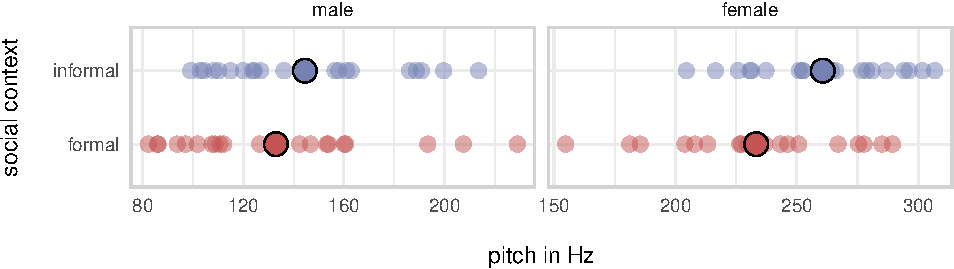
\includegraphics[keepaspectratio]{manuscript_files/figure-pdf/fig-descriptive-dataviz-1.pdf}}

}

\end{figure}%

\subsection{A Bayesian regression model to address our research
question}\label{a-bayesian-regression-model-to-address-our-research-question}

Let us build a Bayesian linear model to approach an answer to this
question. Using the package \texttt{brms}
(\citeproc{ref-Burkner2018-Advanced-Bayesi}{Bürkner, 2018}), our first
step is to specify the model formula and check which priors need to be
specified:

\begin{Shaded}
\begin{Highlighting}[]
\CommentTok{\# contrast code predictor}

\FunctionTok{contrasts}\NormalTok{(polite}\SpecialCharTok{$}\NormalTok{context) }\OtherTok{\textless{}{-}} \FunctionTok{c}\NormalTok{(}\SpecialCharTok{{-}}\FloatTok{0.5}\NormalTok{,}\FloatTok{0.5}\NormalTok{)}

\CommentTok{\# define linear model formula}
\CommentTok{\# predict pitch by context and allow for that relationship }
\CommentTok{\# to vary between subjects}
\NormalTok{formula }\OtherTok{\textless{}{-}} \FunctionTok{bf}\NormalTok{(pitch }\SpecialCharTok{\textasciitilde{}}\NormalTok{ context }\SpecialCharTok{+}\NormalTok{ (}\DecValTok{1} \SpecialCharTok{+}\NormalTok{ context }\SpecialCharTok{|}\NormalTok{ subject))}

\CommentTok{\# get priors for this model}
\FunctionTok{get\_prior}\NormalTok{(formula, polite)[}\FunctionTok{c}\NormalTok{(}\DecValTok{2}\NormalTok{,}\DecValTok{5}\NormalTok{,}\DecValTok{10}\NormalTok{,}\DecValTok{8}\NormalTok{,}\DecValTok{9}\NormalTok{,}\DecValTok{4}\NormalTok{),}\DecValTok{1}\SpecialCharTok{:}\DecValTok{4}\NormalTok{]}
\end{Highlighting}
\end{Shaded}

\begin{verbatim}
                     prior     class      coef   group    source
                    (flat)         b  context1         (unknown)
 student_t(3, 241.5, 35.6) Intercept                   (unknown)
     student_t(3, 0, 35.6)     sigma                   (unknown)
                    (flat)        sd  context1 subject (unknown)
                    (flat)        sd Intercept subject (unknown)
                    (flat)       cor           subject (unknown)
\end{verbatim}

\begin{Shaded}
\begin{Highlighting}[]
\CommentTok{\# }\AlertTok{NOTE}\CommentTok{: make the above prettier? (how to suppress the \textasciigrave{}source\textasciigrave{} column?)}
\end{Highlighting}
\end{Shaded}

The default priors that \texttt{brms} picks for the Intercept and the
variance parameters are mostly reasonable as they are derived from the
data, weakly informative and symmetrical. However the prior for our
critical parameter \texttt{context1} should also be weakly informative
(\citeproc{ref-gelman-etal_Prior_journalarticle_2017}{Gelman et al.,
2017}), i.e.~the prior assumption about the difference between informal
and formal contexts should be that we don't know, but our best guess is
that it is close to zero and equally likely to be more or less than
zero. So we specify a normal distribution centered on zero for this
parameter. (NB: We use default priors for the other parameters for
convenience here, but you should always critically reflect on all of
your priors.)

\begin{Shaded}
\begin{Highlighting}[]
\CommentTok{\# pick a weakly informative prior for the critical parameter}
\NormalTok{priors }\OtherTok{\textless{}{-}} \FunctionTok{prior}\NormalTok{(}\FunctionTok{normal}\NormalTok{(}\DecValTok{0}\NormalTok{, }\DecValTok{20}\NormalTok{), }
                \AttributeTok{class =}\NormalTok{ b, }
                \AttributeTok{coef =} \StringTok{"context1"}\NormalTok{)}
\end{Highlighting}
\end{Shaded}

Now we do a so-called prior predictive check, in other words we want to
know what the posterior distribution looks like before having seen the
data, based on the priors only. This is a useful exercise to make sure
that the priors results in reasonable quantitative assumptions. We
usually do it for all parameters, but here we will focus only on the
critical parameter \texttt{context1}, i.e.~the difference between formal
and informal contexts. Let us also have a look at the predictions for
the prior-only model.

\begin{Shaded}
\begin{Highlighting}[]
\CommentTok{\# }\AlertTok{NOTE}\CommentTok{: CAN WE STORE THE SAMPLING PARAMETERS (seed, iter, chains, cores, backend, data) }
\CommentTok{\# }\AlertTok{NOTE}\CommentTok{: Done for \textquotesingle{}cores\textquotesingle{} and \textquotesingle{}backend\textquotesingle{}, but for the rest we\textquotesingle{}d have to define a custom }
\CommentTok{\#       brms{-}function but that\textquotesingle{}s likely less reader friendly.}

\CommentTok{\# run the model}
\NormalTok{fit\_prior }\OtherTok{\textless{}{-}} \FunctionTok{brm}\NormalTok{(formula, }\AttributeTok{prior =}\NormalTok{ priors, }\AttributeTok{data =}\NormalTok{ polite,}
           \CommentTok{\# sample prior only}
           \AttributeTok{sample\_prior =} \StringTok{"only"}\NormalTok{,}
           \CommentTok{\# store / load model output}
           \AttributeTok{file  =} \StringTok{"../models/fit\_prior"}\NormalTok{,}
           \CommentTok{\# common sampling specifications}
           \AttributeTok{seed =} \DecValTok{1234}\NormalTok{, }\AttributeTok{iter =} \DecValTok{8000}
\NormalTok{           )}
\end{Highlighting}
\end{Shaded}

\begin{figure}[!tbp]

\caption{\label{fig-plot-priors}Prior probability of the effect of
context on pitch, i.e.~before seeing the data}

\centering{

\pandocbounded{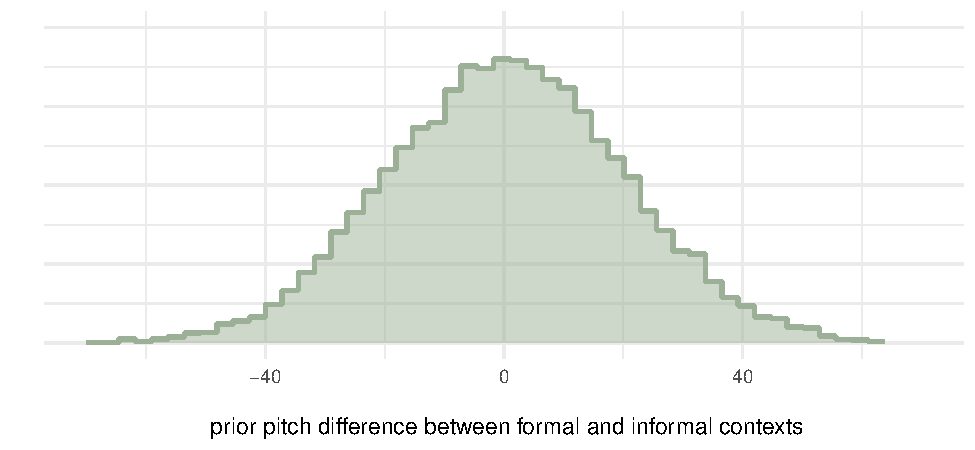
\includegraphics[keepaspectratio]{manuscript_files/figure-pdf/fig-plot-priors-1.pdf}}

}

\end{figure}%

Looking at the distribution in Figure~\ref{fig-plot-priors}, the priors
for the effect of context on pitch seems sensible. The most plausible
value is zero. Values that are smaller or larger than zero become less
plausible the further they are away from zero and values being smaller
or larger than zero are equally likely. Good. Before we have seen the
data, our model is somewhat pessimistic about the effect of context on
on pitch. Now we can run the full model that integrates the likelihood
(our data) with the priors and visualize the posteriors for the critical
parameter.

\begin{Shaded}
\begin{Highlighting}[]
\CommentTok{\# run the model}
\NormalTok{fit }\OtherTok{\textless{}{-}} \FunctionTok{brm}\NormalTok{(formula, }\AttributeTok{prior =}\NormalTok{ priors, }\AttributeTok{data =}\NormalTok{ polite,}
           \CommentTok{\# store / load model output}
           \AttributeTok{file  =} \StringTok{"../models/fit"}\NormalTok{,}
           \CommentTok{\# common sampling specifications}
           \AttributeTok{seed =} \DecValTok{1234}\NormalTok{, }\AttributeTok{iter =} \DecValTok{8000}
\NormalTok{           )}
\end{Highlighting}
\end{Shaded}

\begin{figure}[!tbp]

\caption{\label{fig-plot-posterior}Posterior probability of the effect
of context on pitch, i.e.~after seeing the data}

\centering{

\pandocbounded{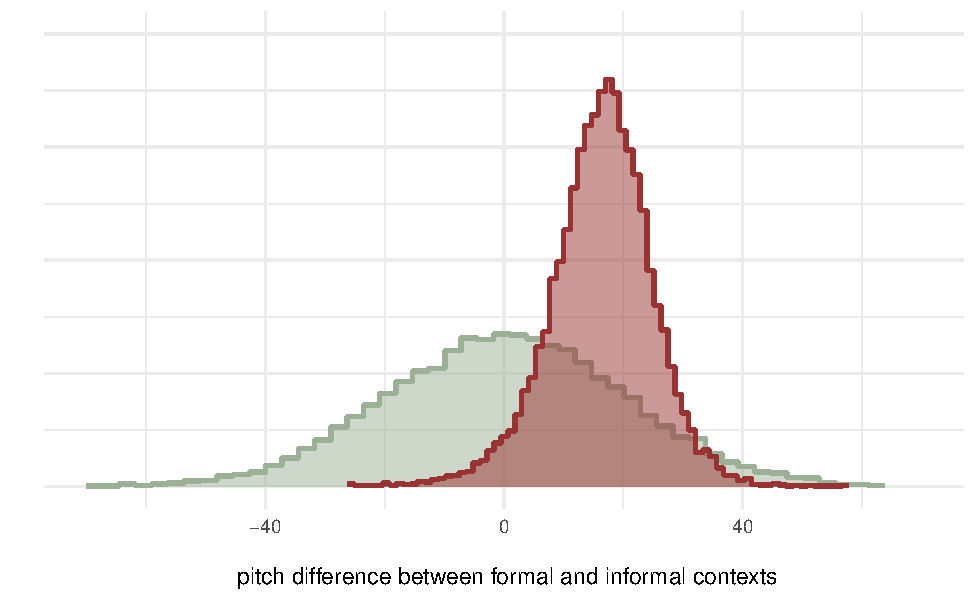
\includegraphics[keepaspectratio]{manuscript_files/figure-pdf/fig-plot-posterior-1.pdf}}

}

\end{figure}%

Figure~\ref{fig-plot-posterior} shows the prior (green distribution) and
posterior (red distribution) probability of the effect of context on
pitch. The distribution of posterior samples (red) suggests that the
majority of plausible values after seeing the data are positive, or in
other words, informal contexts elicit larger pitch values. Negative
values are not very plausible posterior values, but also not completely
implausible. Compared to our prior probability (green distribution) for
which roughly 50\% of posteriors are negative, this decrease in
plausibility of negative values is quite noteworthy already.

What we have done here should be quite familiar. We compare our model
predictions to a reference point. It is a single point value: zero. But
do we really care that much for such point hypotheses? Is zero really
that special? We might think so because years of using null hypothesis
significance testing has conditioned us to think that way. But this
tutorial would like to break this cycle and move forward. Bear with us
and let's approach hypothesis testing a bit differently today.

\subsection{Grounding hypotheses in regions of practical
equivalences}\label{grounding-hypotheses-in-regions-of-practical-equivalences}

Above we claimed that we wanted to test ``whether pitch is
\textbf{meaningfully affected} by the social context of the utterance''.
We snuck the word meaningfully in there for a reason. But what does
``meaningful'' mean? This is an interesting yet deep questions and
(un)fortunately requires quite a bit of thinking. As we argue here, what
a meaningful difference is, depends on the context of the data. So let's
have a closer look at our data.

This tutorial deals with speech data. Speech is, in spoken languages at
least, \emph{the} vehicle to transmit linguistic information in order to
communicate with each other. Speech is also very complex and very noisy:
Not everything that can be measured in the acoustic signal matters for
the listener. For example, if something cannot be perceived reliably, it
is at least conceivable that it might play little to no role in
communication. While the speech sciences have a rich research tradition
to estimate what can and what cannot be reliably heard, exact estimation
depends on a lot of moving parts. Such thresholds are referred to as
\emph{Just Noticeable Differences} (JNDs) and can be used to define what
constitutes meaningful differences when we look at speech data.

For example, Liu (\citeproc{ref-liu2013just}{2013}) report on JNDs
ranging from 3 to 14 Hz. Jongman et al.
(\citeproc{ref-jongman2017just}{2017}) report on JNDs between 6 and 9
Hz. Turner et al. (\citeproc{ref-turner2019perception}{2019}) reported
on JNDs between 17 and 25 Hz for non-speech stimuli and between 35 and
40 Hz for speech stimuli. While these studies are hard to compare, they
give us at least an idea about the rough order of magnitude for JND
values to work with when it comes to speech data like the data set at
hand.

Based on these considerations, we could interpret the original
hypothesis the following way: If a pitch difference is below the JND, it
is not meaningful. So, instead of testing against a point-valued
hypothesis, we can test against a range of parameter values that are
equivalent to the null value for practical purposes. In our case, let us
begin with the lowest reported JND of the above studies on pitch
perception in speech (3 Hz), but be extra conservative and double the
reported JND to 6 Hz. We then assume that pitch values between
\texttt{-6} and \texttt{6} are meaningless. Such ranges are sometimes
called \emph{regions of practical equivalence} (ROPEs), range of
equivalence, equivalence margin, smallest effect size of interest, or
good-enough belt (see
\citeproc{ref-kruschke_Rejecting_journalarticle_2018}{Kruschke, 2018}).

\begin{Shaded}
\begin{Highlighting}[]
\NormalTok{rope }\OtherTok{\textless{}{-}} \FunctionTok{c}\NormalTok{(}\SpecialCharTok{{-}}\DecValTok{6}\NormalTok{,}\DecValTok{6}\NormalTok{)}
\end{Highlighting}
\end{Shaded}

With a ROPE being defined, we can now test our hypothesis ``whether
pitch is \textbf{meaningfully affected} by the social context of the
utterance'' using Bayes Factors.

\section{Testing hypothesis using Bayes
Factor}\label{testing-hypothesis-using-bayes-factor}

\subsection{What is Bayes Factor?}\label{what-is-bayes-factor}

Suppose we have two hypotheses \(H_0\) and \(H_1\) and want to know
which of these is correct. We do so by looking at some observed data
\(D\). As Bayesians, the first most obvious thing to look at is how
likely each hypothesis is after seeing the data, i.e., something like
\(P(H_0 \mid D)\) and \(P(H_1 \mid D)\). Now, it turns out that these
\emph{posterior probabilities of hypotheses} are problematic, because
they depend on the prior probabilities of the hypotheses \(P(H_0)\) and
\(P(H_1)\), which are often hard to justify. To see this, imagine that
the hypotheses on the table are deep issues like a contrast between
Darwinian evolutionary theory and intelligent design. Proponents of
either view would have a hard time agreeing on priors for these
hypotheses, but may find it much easier to agree on which observations
are made more or less likely by either hypothesis. Therefore, the
preferred Bayesian measure is the Bayes factor, which is defined as the
likelihood ratio of the data given each hypothesis:

\[
\text{Bayes factor in favor of hypothesis 1 over hypothesis 2} \ \  \colon\!= \ \ \frac{P(D \mid H_1)}{P(D \mid H_0)}
\]

To see how this is an objective and actually quite intuitive measure of
observational evidence in scientific reasoning, consider the case of
Darwinian evolution (\(H_1\)) versus intelligent design \(H_0\) again.
Let's take the historical case of observing how the beak sizes of
finches on the Galápagos islands changed over time as a functional
adaptation to environmental changes. What is a better explanation of
that observation? To begin with, let's notice that this observation is
\emph{not} ruled out by either hypothesis. But the probability of
observing \(D\) (adaptively changing beak sizes) is much higher under
Darwinian evolution than under intelligent design. This is because the
latter is compatible with many more counterfactual observations, such as
beak sizes staying the same over time, or even beak sizes changing in a
way that is not adaptive. So, the probability of the observed data is
much higher under Darwinian evolution than under intelligent design, so
that \(P(D \mid H_1) > P(D \mid H_0)\), irrespective of what we
initiallly believed is the correct hypothesis. This is what corroborates
the intuition that the observation \(D\) is an argument in favor of
\(H_1\) and not \(H_0\), and this is exactly what the Bayes factor
quantifies.

Concretely, a Bayes factor of 1 corresponds to the case of
\(P(D \mid H_1) = P(D \mid H_0)\), i.e., the data is equally likely
under both hypotheses, so the data does not provide any evidence for or
against either hypothesis. Any Bayes factor larger than 1 indicates that
the data is more likely under \(H_1\) than under \(H_0\), and the larger
the Bayes factor, the stronger the evidence in favor of \(H_1\).
Conversely, any Bayes factor smaller than 1 indicates that the data is
more likely under \(H_0\) than under \(H_1\). Notice that the Bayes
factor is symmetric in the sense that a Bayes factor of 3 in favor of
\(H_1\) over \(H_0\) corresponds to a Bayes factor of 1/3 in favor of
\(H_0\) over \(H_1\). There are various conventions for interpreting the
strength of evidence of Bayes factors, such as to consider as
``\emph{mild evidence}'' Bayes factors bigger than 3, ``\emph{strong
evidence}'' Bayes factors bigger than 10, and ``\emph{decisive
evidence}'' Bayes factors bigger than 30.

One way to interpret Bayes factors in absolute terms is this. A Bayes
factor of \(n\) in favor of \(H_1\) over \(H_0\) means that after seeing
the data, a rational researcher who thought both hypotheses were equally
likely would consider \(H_1\) to be \(n\) times more likely than \(H_0\)
after observing \(D\). In other words, if you are maximally uncertain
before, then observe \(D\) and that makes you weight \(H_1\) \(n\) times
more than \(H_0\), then the Bayes factor is \(n\).

\subsection{Bayes factors for statistical
models}\label{bayes-factors-for-statistical-models}

After motivating Bayes factors in general, let's have a look at the
definition of Bayes factors in the context of statistical models. This
small section is a bit more technical, but it can be skipped without too
much loss.

In the context of statistical models, we can use Bayes factors to
compare two statistical models \(M_0\) and \(M_1\) that instantiate two
competing hypotheses (or assumptions) \(H_0\) and \(H_1\). A Bayesian
statistical model \(M\) consists of:

\begin{enumerate}
\def\labelenumi{\arabic{enumi}.}
\tightlist
\item
  a \emph{likelihood function} \(P(D \mid \theta, M)\) that specifies
  how likely the observed data \(D\) is given the model \(M\) and the
  model's parameters \(\theta\), and
\item
  a \emph{prior distribution} \(P(\theta \mid M)\) that specifies how
  likely different parameter values are before seeing the data.
\end{enumerate}

The probability of some observed data \(P(D \mid M)\) under a model
\(M\) is then obtained by integrating over all possible parameter values
\(\theta\):

\[
P(D \mid M) = \int P(D \mid \theta, M) \ \  P(\theta \mid M) d\theta
\]

This is called the \emph{marginal likelihood} of the data under the
model \(M\). We can think of this quantity as obtained from sampling
repeatedly parameter values from the prior and then sampling, for of
these, a potential data observation. (Notice that this is the
\emph{prior predictive data distribution} of the model.)

Putting things together, the resulting definition for Bayes factors in
statistical models is:

\[
\text{Bayes factor in favor of model 1 over model 2} \ \  \colon\!= \ \ \frac{P(D \mid M_1)}{P(D \mid M_0)} = \frac{\int P(D \mid \theta, M_1) \ \  P(\theta \mid M_1) d\theta}{\int P(D \mid \theta, M_0) \ \  P(\theta \mid M_0) d\theta}
\]

\subsection{Approximating Bayes Factor with the Savage-Dickey method
(for point-valued
hypotheses)}\label{approximating-bayes-factor-with-the-savage-dickey-method-for-point-valued-hypotheses}

While Bayes factors are a very intuitive and useful measure of evidence,
they are often hard to compute. There are various approximation methods,
such as bridge sampling
(\citeproc{ref-GronauSarafoglou2017-A-tutorial-on-b}{Gronau et al.,
2017}), which can be used for any arbitrary pair of models, but these
can still be computationally costly and sometimes hard to implement.
However, for the special case of \emph{nested models}, there is a simple
and computationally cheap approximation method called the
\emph{Savage-Dickey density ratio}
(\citeproc{ref-DickeyLientz1970-The-Weighted-Li}{Dickey \& Lientz,
1970};
\citeproc{ref-WagenmakersLodewyckx2010-Bayesian-hypoth}{Wagenmakers et
al., 2010}).

Intuitively speaking, model \(M_0\) is nested in model \(M_1\) if
\(M_0\) can be obtained from \(M_1\) by fixing one or more parameters to
a specific value. For example, we may consider a model \(M_1\) that has
a normal distribution on the \texttt{context} coefficient as a prior,
and a nested model \(M_0\) that has a degenerate prior on the
\texttt{context} coefficient that puts all its mass on zero. That model
\(M_0\) would then correspond to the (standard, point-valued) null
hypothesis that there is no effect of \texttt{context} on
\texttt{pitch}.

So, suppose that \(M_0\) is nested in \(M_1\) by fixing a critical
parameter \(\theta^*\) to a specific value \(x\). Then, the
Savage-Dickey density ratio states that the Bayes factor in favor of
\(M_1\) over \(M_0\) can be computed as the ratio of the prior and
posterior density of the critical parameter at the point value that
defines the null hypothesis:

\[
\text{Bayes factor in favor of model 1 over model 2} \ \  = \ \  \frac{P(\theta^*=x \mid D, M_1)}{P(\theta^*=x \mid M_1)}
\] Let's unpack this. First of all, this seemingly magical result is
actually not that magical, but follows directly from the definition of
Bayes factors and Bayes' theorem, but we skip the derivation here. What
this means is that in practice we do not have to calculate or
approximate any integrals at all, but we can simply look at one model
and run posterior inference, like we routinly do with \texttt{brms}, for
example. Look at the formula above: we would only need to run one model,
\(M_1\), and then look at the prior and posterior density of the
critical parameter \(\theta^*\) at the point value \(x\). The prior, we
should usually be able to get easily because it is in our hands to
specify it. The posterior probably, we could get by estimating it from
the samples that are returned by software like \texttt{brms} \ldots{}

\ldots{} well, at least in principle. One problem here is that
estimating \(P(\theta^*=x \mid D, M_1)\) from posterior samples is
fickle. We can do it with some mathematical methods, but we may need a
lot of samples and do some post-processing (e.g., using splines). The
main point is that posterior samples are not reliable for estimating
densities at specific points, but they are reliable for estimating
probabilities over ranges of values. Ah, if only there was a
generalization of the Savage-Dickey density ratio that works for ranges
of values!

Wait: there is!

\subsection{Calculating Bayes Factor for a specified Region of Practical
Equivalence
(ROPE)}\label{calculating-bayes-factor-for-a-specified-region-of-practical-equivalence-rope}

The Bayes Factor in favor of model \(M_{0}\) over alternative model
\(M_{1}\) is: \[
BF_{01} = \frac{P(\theta \in I_{0} \mid D, M_{e})}{P(\theta \in I_{1} \mid D, M_{e})} \ \frac{P(\theta \in I_{1} \mid  M_{e})}{P(\theta \in I_{0} \mid M_{e})}
\]

Figure~\ref{fig-savage-dickey} shows \ldots{}

\begin{figure}[!tbp]

\caption{\label{fig-savage-dickey}}

\centering{

\pandocbounded{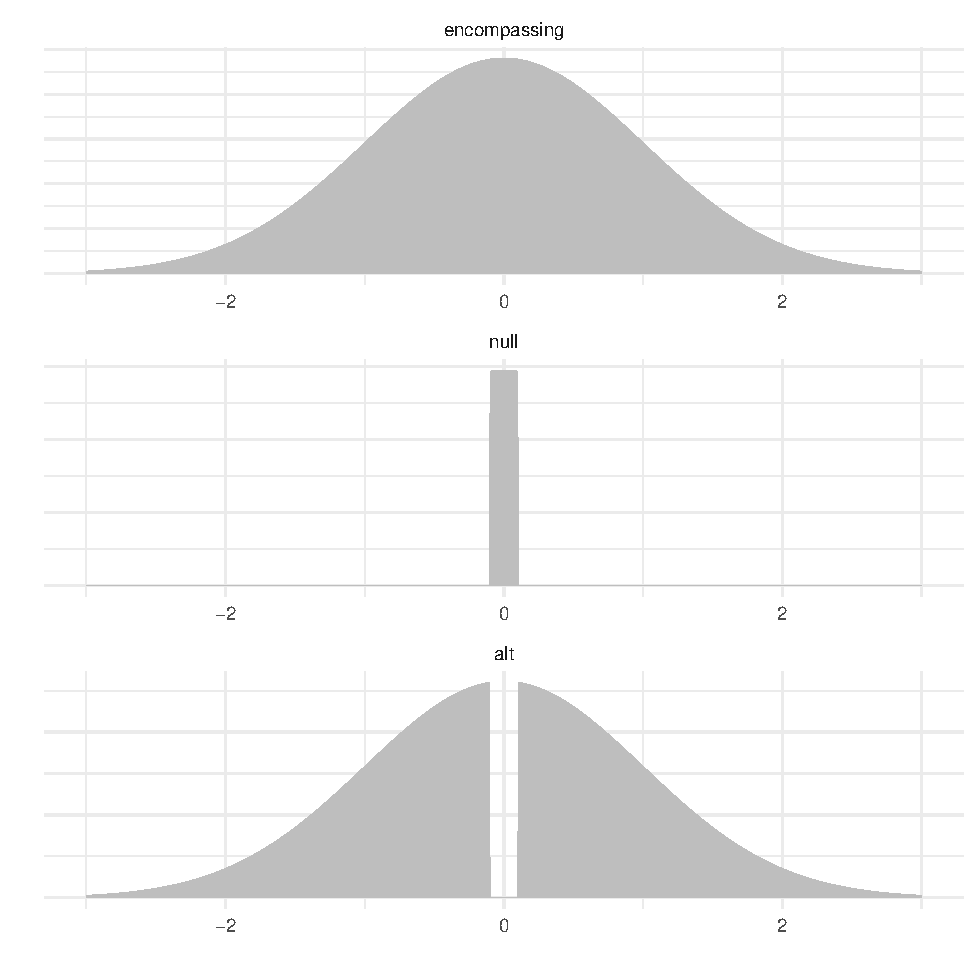
\includegraphics[keepaspectratio]{manuscript_files/figure-pdf/fig-savage-dickey-1.pdf}}

}

\end{figure}%

Instead of doing it by hand, we can calculate the Savage Dickey ratio
with the \texttt{bayesfactor\_parameters()} function from the
\texttt{bayesfactorR} package. What happens behind the scenes is that
the function will sample posteriors from your specified model based on
priors only (so before seeing any data) and calculates the posterior
probability of the specified \texttt{null} hypothesis (here the range
specified by our ROPE).

\begin{Shaded}
\begin{Highlighting}[]
\CommentTok{\#|warning: FALSE}
\CommentTok{\#|message: FALSE}

\NormalTok{BF\_1 }\OtherTok{\textless{}{-}} \FunctionTok{bayesfactor\_parameters}\NormalTok{(}\AttributeTok{posterior =}\NormalTok{ fit, }
                               \AttributeTok{null =}\NormalTok{ rope, }
                               \AttributeTok{parameter =} \StringTok{"b\_context1"}\NormalTok{)}
\end{Highlighting}
\end{Shaded}

Before interpreting the number we get, let us visually explore what our
BF corresponds to.

\begin{Shaded}
\begin{Highlighting}[]
\NormalTok{posterior\_plot }\SpecialCharTok{+} 
  \FunctionTok{geom\_vline}\NormalTok{(}\AttributeTok{xintercept =} \FunctionTok{c}\NormalTok{(rope[}\DecValTok{1}\NormalTok{], rope[}\DecValTok{2}\NormalTok{]),}
             \AttributeTok{lty =} \StringTok{"dashed"}\NormalTok{)}
\end{Highlighting}
\end{Shaded}

\begin{figure}[!tbp]

\caption{Prior and posterior probability of the effect of context on
pitch relative to the ROPE (-0.1, 0.1)}

{\centering \pandocbounded{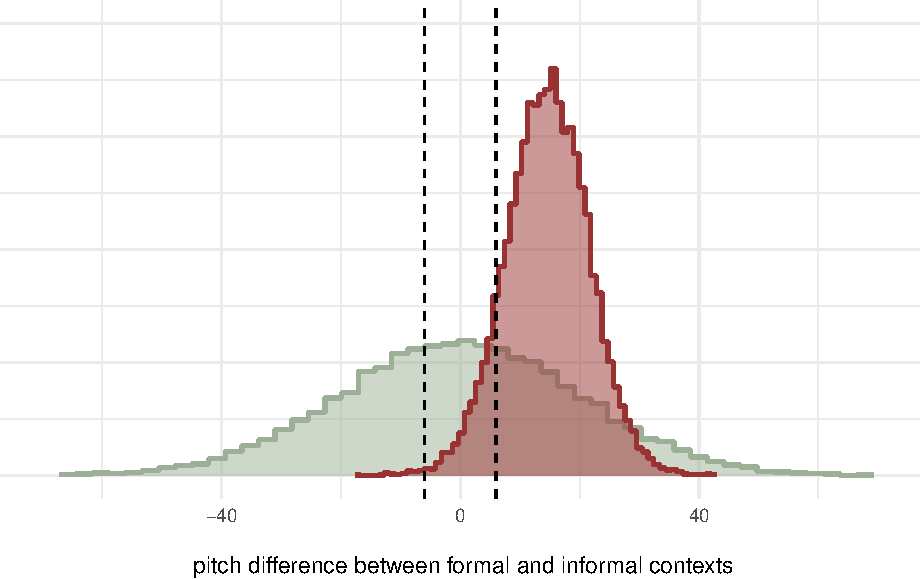
\includegraphics[keepaspectratio]{manuscript_files/figure-pdf/plot-ropes-1.pdf}}

}

\end{figure}%

What the BF does is relating two numbers: (a) The prior probability of
parameter values outside the rope, i.e.~the proportion of the green
distribution that falls outside the dashed lines, and (b) the posterior
probability of parameter values outside the rope, i.e.~the proportion of
the red distribution that falls outside the dashed lines. Eye-balling
the plot, we can maybe already see that more of the red distribution is
outside the ROPE than of the green distribution.

\begin{Shaded}
\begin{Highlighting}[]
\NormalTok{BF\_1}
\end{Highlighting}
\end{Shaded}

\begin{verbatim}
Bayes Factor (Null-Interval)

Parameter |   BF
----------------
context1  | 2.88

* Evidence Against The Null: [-6.000, 6.000]
\end{verbatim}

To be exact, 2.7 times for of the red distribution is outside of the
ROPE than of the green distribution.

That means the model that has seen the data provide 2.7 times more
evidence for pitch being outside of the ROPE, or in other words, it is
2.7 times more likely (after having seen the data), that context affects
pitch meaningfully. According to Lee and Wagenmakers
(\citeproc{ref-lee-wagenmakers_Bayesian_book_2014}{2014}) criteria for
interpreting BFs, this value corresponds to only anecdotal evidence for
the alternative hypothesis.

\subsection{Sensitivity analysis for different priors and
ROPEs}\label{sensitivity-analysis-for-different-priors-and-ropes}

Now as you probably have guessed already, all these probabilities are
very much dependent on the priors of the model, so it is important to
evaluate the robustness of our Bayes Factor-based interpretation across
a range of sensible priors. And as long as we are not a 100\% sure about
what a meaningful difference is, we might as well explore the robustness
of the Bayes Factor across different ROPEs. We won't bore you with the
code for that process, but you can follow it along in our scripts. Let
us explore the following ROPE intervals as informed by the three studies
cited above on pitch perception: we test a range of ROPE intervals from
6 Hz to 40 Hz. We also assume the following five prior values for the
width of the standard deviation of the critical parameter (centered on
zero): 10, 15, 20, 25, 30. These are all sensible prior widths assuming
that medium to strong effects in either direction are plausible.

\begin{figure}[!tbp]

\caption{Bayes Factors for a range of priors and a range of ROPEs}

{\centering \pandocbounded{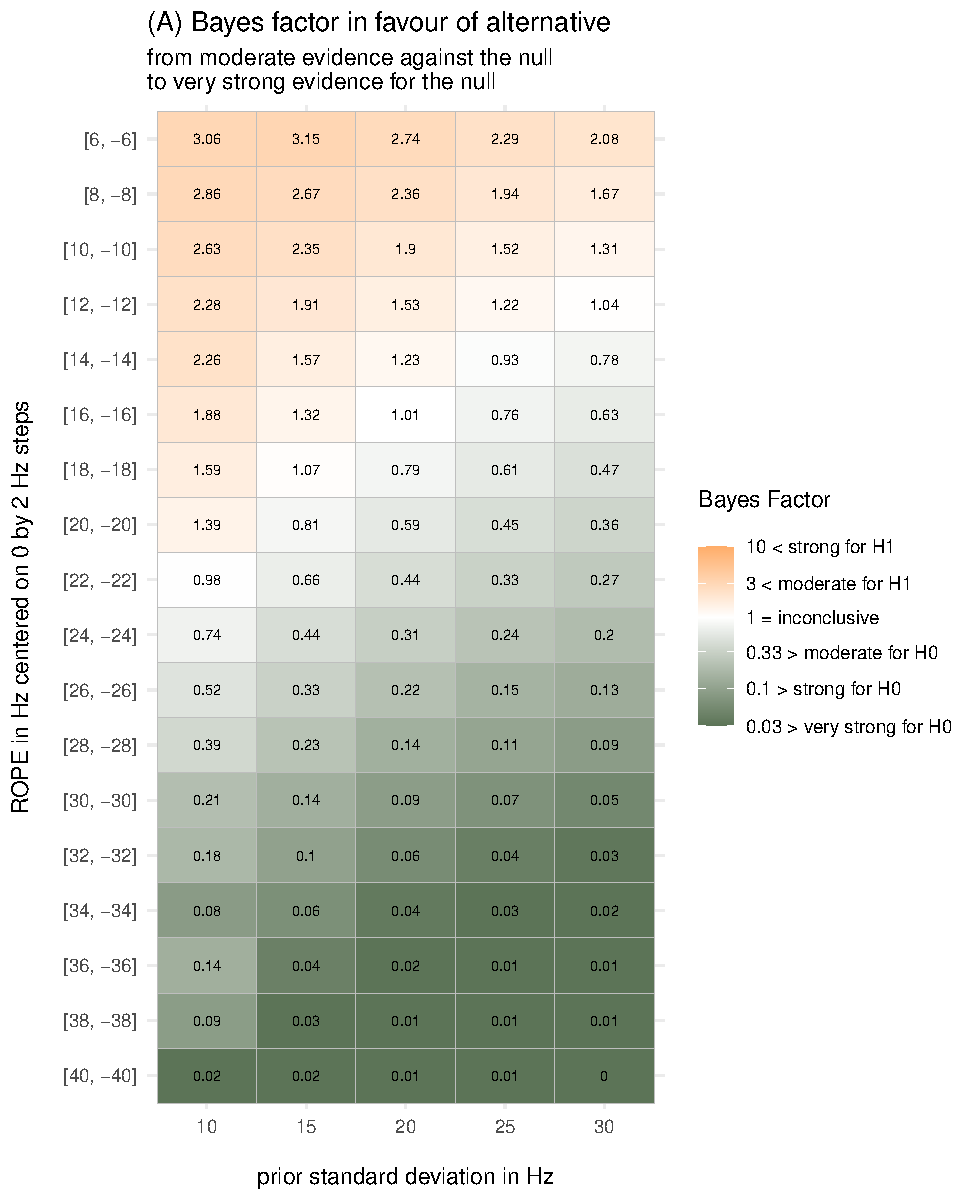
\includegraphics[keepaspectratio]{manuscript_files/figure-pdf/visualize-raster-1.pdf}}

}

\end{figure}%

The combination of Bayes Factors is visualized in Figure X. Orange cells
indicate evidence for the alternative. Green cells indicate evidence for
the null. It becomes clear that the conclusions we can draw from our
data are rather dependent on the choices we made along the way.

By comparing the Bayes Factors along the y-axis, we can see that they
are heavily dependent on the chosen ROPE. We here chose (theoretically
speaking) a quite large range of ROPEs, all of which are informed by
psychoacoustic studies of what pitch differences can be reliably heard
and thus likely are meaningful for communication. In light of this range
of possible definitions what constitutes meaningful differences, our
data seem not very robust, as illustrated by the shift from orange to
green. Even the smallest ROPE intervals provide only anecdotal to
moderate evidence for the alternative. And the most conservative ROPEs,
following Turner et al. (\citeproc{ref-turner2019perception}{2019}),
leads to moderate to very strong evidence against the alternative
hypothesis.

Additionally, when comparing the Bayes Factors along the x-axis, we can
see that they are comparatively consistent for different standard
deviations of the critical prior. However, we can also see that the
Bayes Factors decrease with the width of the priors (from left to
right). This is not surprising and a known phenomenon, often discussed
under the Jeffreys-Lindley paradox
(\citeproc{ref-lindley_Statistical_journalarticle_1957}{Lindley, 1957}):
The more diffuse the priors are (i.e.~wider priors), the larger is the
probability that a specific parameter values is not compatible with the
data.

Combined, we can see that the larger the ROPE and the wider the priors,
the more likely becomes the null hypothesis. In an ideal world, the
evidence provided by the data should be robust across these choices.
However, this exploration of our inference is a fantastic opportunity to
assess the boundaries of our conclusions. In this case, the original
conclusions by Winter and Grawunder
(\citeproc{ref-winter-grawunder_Phonetic_journalarticle_2012}{2012}) was
based on the null hypothesis significance testing and traditionally
tested the compatibility of the data with a point-null hypothesis. They
concluded ``that in formal speech, Korean {[}\ldots{]} female speakers
lowered their average fundamental frequency {[}\ldots{]}.'' This
statement is still true according to their inferential criteria, but
thinking more deeply about the theoretical consequences of differences
in pitch, it might be less clear that these differenecs are truly
meaninful.

\subsection{BF for point hypothesis}\label{bf-for-point-hypothesis}

don't lol

\section{How to write things up}\label{how-to-write-things-up}

\section{Some words of encouragement}\label{some-words-of-encouragement}

Bayesian inference in general and this form of hypothesis testing in
particular require much more thinking than we might be used to. We think
this is a good thing. Many voices have criticized the lack of engagement
that we behavioral scientists invest into thinking how our theoretical
ideas connect to concrete predictions in the quantitative systems under
investigation (\citeproc{ref-coretta2023multidimensional}{Coretta et
al., 2023}; e.g. \citeproc{ref-scheel2022most}{Scheel, 2022};
\citeproc{ref-woensdregt2024lessons}{Woensdregt et al., 2024}). The
presented form of hypothesis testing is easy to understand, but does
require to think deeply about prior quantitative assumptions as well as
what it means for observations to be meaningfully different. That is
neither trivial nor easy. But we would like to encourage you to engage
in exactly this thinking to better understand our data and how they
might link with our understanding of cognition and behavior.

\section{Other Resources}\label{other-resources}

There are many fantastic resources out there to help you learn about the
wonderful world of statistics. Here are a few recommendations. - A very
accessible introduction to linear models in R is Winter
(\citeproc{ref-winter2019statistics}{2019}). - \ldots{}

\section{References}\label{references}

\begin{verbatim}
R version 4.5.1 (2025-06-13)
Platform: aarch64-apple-darwin20
Running under: macOS Sequoia 15.6

Matrix products: default
BLAS:   /Library/Frameworks/R.framework/Versions/4.5-arm64/Resources/lib/libRblas.0.dylib 
LAPACK: /Library/Frameworks/R.framework/Versions/4.5-arm64/Resources/lib/libRlapack.dylib;  LAPACK version 3.12.1

locale:
[1] en_US.UTF-8/en_US.UTF-8/en_US.UTF-8/C/en_US.UTF-8/en_US.UTF-8

time zone: Europe/Amsterdam
tzcode source: internal

attached base packages:
[1] stats     graphics  grDevices utils     datasets  methods   base     

other attached packages:
 [1] bayestestR_0.16.1 tidybayes_3.0.7   brms_2.22.0       Rcpp_1.1.0       
 [5] ggdist_3.3.3      lubridate_1.9.4   forcats_1.0.0     stringr_1.5.1    
 [9] dplyr_1.1.4       purrr_1.1.0       readr_2.1.5       tidyr_1.3.1      
[13] tibble_3.3.0      ggplot2_3.5.2     tidyverse_2.0.0  

loaded via a namespace (and not attached):
 [1] gtable_0.3.6         tensorA_0.36.2.1     xfun_0.53           
 [4] insight_1.4.0        processx_3.8.6       lattice_0.22-7      
 [7] tzdb_0.5.0           vctrs_0.6.5          tools_4.5.1         
[10] ps_1.9.1             generics_0.1.4       parallel_4.5.1      
[13] cmdstanr_0.9.0       pkgconfig_2.0.3      Matrix_1.7-3        
[16] checkmate_2.3.3      RColorBrewer_1.1-3   distributional_0.5.0
[19] RcppParallel_5.1.10  lifecycle_1.0.4      compiler_4.5.1      
[22] farver_2.1.2         Brobdingnag_1.2-9    tinytex_0.57        
[25] codetools_0.2-20     htmltools_0.5.8.1    bayesplot_1.13.0    
[28] yaml_2.3.10          crayon_1.5.3         pillar_1.11.0       
[31] arrayhelpers_1.1-0   bridgesampling_1.1-2 abind_1.4-8         
[34] nlme_3.1-168         posterior_1.6.1      tidyselect_1.2.1    
[37] digest_0.6.37        svUnit_1.0.6         mvtnorm_1.3-3       
[40] stringi_1.8.7        fastmap_1.2.0        grid_4.5.1          
[43] cli_3.6.5            magrittr_2.0.3       loo_2.8.0           
[46] withr_3.0.2          scales_1.4.0         backports_1.5.0     
[49] bit64_4.6.0-1        timechange_0.3.0     rmarkdown_2.29      
[52] matrixStats_1.5.0    bit_4.6.0            hms_1.1.3           
[55] coda_0.19-4.1        evaluate_1.0.4       knitr_1.50          
[58] rstantools_2.4.0     rlang_1.1.6          glue_1.8.0          
[61] vroom_1.6.5          rstudioapi_0.17.1    jsonlite_2.0.0      
[64] R6_2.6.1            
\end{verbatim}

\begin{verbatim}
[[1]]
Bürkner P (2017). "brms: An R Package for Bayesian Multilevel Models
Using Stan." _Journal of Statistical Software_, *80*(1), 1-28.
doi:10.18637/jss.v080.i01 <https://doi.org/10.18637/jss.v080.i01>.

Bürkner P (2018). "Advanced Bayesian Multilevel Modeling with the R
Package brms." _The R Journal_, *10*(1), 395-411.
doi:10.32614/RJ-2018-017 <https://doi.org/10.32614/RJ-2018-017>.

Bürkner P (2021). "Bayesian Item Response Modeling in R with brms and
Stan." _Journal of Statistical Software_, *100*(5), 1-54.
doi:10.18637/jss.v100.i05 <https://doi.org/10.18637/jss.v100.i05>.

[[2]]
Makowski D, Ben-Shachar M, Lüdecke D (2019). "bayestestR: Describing
Effects and their Uncertainty, Existence and Significance within the
Bayesian Framework." _Journal of Open Source Software_, *4*(40), 1541.
doi:10.21105/joss.01541 <https://doi.org/10.21105/joss.01541>,
<https://joss.theoj.org/papers/10.21105/joss.01541>.

[[3]]
Kay M (2024). _tidybayes: Tidy Data and Geoms for Bayesian Models_.
doi:10.5281/zenodo.1308151 <https://doi.org/10.5281/zenodo.1308151>, R
package version 3.0.7, <http://mjskay.github.io/tidybayes/>.

[[4]]
Wickham H, Averick M, Bryan J, Chang W, McGowan LD, François R,
Grolemund G, Hayes A, Henry L, Hester J, Kuhn M, Pedersen TL, Miller E,
Bache SM, Müller K, Ooms J, Robinson D, Seidel DP, Spinu V, Takahashi
K, Vaughan D, Wilke C, Woo K, Yutani H (2019). "Welcome to the
tidyverse." _Journal of Open Source Software_, *4*(43), 1686.
doi:10.21105/joss.01686 <https://doi.org/10.21105/joss.01686>.

[[5]]
Kay M (2024). "ggdist: Visualizations of Distributions and Uncertainty
in the Grammar of Graphics." _IEEE Transactions on Visualization and
Computer Graphics_, *30*(1), 414-424. doi:10.1109/TVCG.2023.3327195
<https://doi.org/10.1109/TVCG.2023.3327195>.

Kay M (2025). _ggdist: Visualizations of Distributions and
Uncertainty_. doi:10.5281/zenodo.3879620
<https://doi.org/10.5281/zenodo.3879620>, R package version 3.3.3,
<https://mjskay.github.io/ggdist/>.
\end{verbatim}

\phantomsection\label{refs}
\begin{CSLReferences}{1}{0}
\bibitem[\citeproctext]{ref-Burkner2018-Advanced-Bayesi}
Bürkner, P.-C. (2018). {Advanced Bayesian Multilevel Modeling with the R
Package brms}. \emph{{The R Journal}}, \emph{10}(1), 395--411.
\url{https://doi.org/10.32614/RJ-2018-017}

\bibitem[\citeproctext]{ref-coretta2023multidimensional}
Coretta, S., Casillas, J. V., Roessig, S., Franke, M., Ahn, B.,
Al-Hoorie, A. H., Al-Tamimi, J., Alotaibi, N. E., AlShakhori, M. K.,
Altmiller, R. M., et al. (2023). Multidimensional signals and analytic
flexibility: Estimating degrees of freedom in human-speech analyses.
\emph{Advances in Methods and Practices in Psychological Science},
\emph{6}(3), 25152459231162567.

\bibitem[\citeproctext]{ref-DickeyLientz1970-The-Weighted-Li}
Dickey, J. M., \& Lientz, B. P. (1970). The weighted likelihood ratio,
sharp hypotheses about chances, the order of a {M}arkov chain. \emph{The
Annals of Mathematical Statistics}, \emph{41}(1), 214--226.

\bibitem[\citeproctext]{ref-franke-roettger_Bayesian_preprint_2019}
Franke, M., \& Roettger, T. (2019). \emph{Bayesian regression modeling
(for factorial designs): {A} tutorial}. OSF.
\url{https://doi.org/10.31234/osf.io/cdxv3}

\bibitem[\citeproctext]{ref-gelman-etal_Prior_journalarticle_2017}
Gelman, A., Simpson, D., \& Betancourt, M. (2017). The {Prior Can Often
Only Be Understood} in the {Context} of the {Likelihood}.
\emph{Entropy}, \emph{19}(10), 555.
\url{https://doi.org/10.3390/e19100555}

\bibitem[\citeproctext]{ref-GronauSarafoglou2017-A-tutorial-on-b}
Gronau, Q. F., Sarafoglou, A., Matzke, D., Ly, A., Boehm, U., Marsman,
M., Leslie, D. S., Forster, J. J., Wagenmakers, E.-J., \& Steingroever,
H. (2017). A tutorial on bridge sampling. \emph{Journal of Mathematical
Psychology}, \emph{81}, 80--97.
\url{https://doi.org/doi.org/10.1016/j.jmp.2017.09.005}

\bibitem[\citeproctext]{ref-jongman2017just}
Jongman, A., Qin, Z., Zhang, J., \& Sereno, J. A. (2017). Just
noticeable differences for pitch direction, height, and slope for
mandarin and english listeners. \emph{The Journal of the Acoustical
Society of America}, \emph{142}(2), EL163--EL169.

\bibitem[\citeproctext]{ref-KassRaftery1995-Bayes-Factors}
Kass, R. E., \& Raftery, A. E. (1995). Bayes factors. \emph{Journal of
the American Statistical Association}, \emph{90}(430), 773--795.

\bibitem[\citeproctext]{ref-KlugkistHoijtink2007-The-Bayes-facto}
Klugkist, I., \& Hoijtink, H. (2007). The bayes factor for inequality
and about equality constrained models. \emph{Computational Statistics
and Data Analysis}, \emph{51}(12), 6367--6379.
\url{https://doi.org/10.1016/j.csda.2007.01.024}

\bibitem[\citeproctext]{ref-KlugkistKato2005-Bayesian-model}
Klugkist, I., Kato, B., \& Hoijtink, H. (2005). Bayesian model selection
using encompassing priors. \emph{Statistica Neelandica}, \emph{59}(1),
57--69.

\bibitem[\citeproctext]{ref-kruschke_Rejecting_journalarticle_2018}
Kruschke, J. K. (2018). Rejecting or {Accepting Parameter Values} in
{Bayesian Estimation}. \emph{Advances in Methods and Practices in
Psychological Science}, \emph{1}(2), 270--280.
\url{https://doi.org/10.1177/2515245918771304}

\bibitem[\citeproctext]{ref-lee-wagenmakers_Bayesian_book_2014}
Lee, M. D., \& Wagenmakers, E.-J. (2014). \emph{Bayesian {Cognitive
Modeling}: {A Practical Course}}. Cambridge University Press.

\bibitem[\citeproctext]{ref-lindley_Statistical_journalarticle_1957}
Lindley, D. V. (1957). A {Statistical Paradox}. \emph{Biometrika},
\emph{44}(1/2), 187--192. \url{https://doi.org/10.2307/2333251}

\bibitem[\citeproctext]{ref-liu2013just}
Liu, C. (2013). Just noticeable difference of tone pitch contour change
for english-and chinese-native listeners. \emph{The Journal of the
Acoustical Society of America}, \emph{134}(4), 3011--3020.

\bibitem[\citeproctext]{ref-MoreyRomeijn2016-philosophyOfBFs}
Morey, R. D., Romeijn, J.-W., \& Rouder, J. N. (2016). The philosophy of
bayes factors and the quantification of statistical evidence.
\emph{Journal of Mathematical Psychology}, \emph{72}, 6--18.
\url{https://doi.org/10.1016/j.jmp.2015.11.001}

\bibitem[\citeproctext]{ref-Oh2014-Bayesian-compar}
Oh, M.-S. (2014). Bayesian comparison of models with inequality and
equality constraints. \emph{Statistics and Probability Letters},
\emph{84}, 176--182. \url{https://doi.org/10.1016/j.spl.2013.10.005}

\bibitem[\citeproctext]{ref-scheel2022most}
Scheel, A. M. (2022). Why most psychological research findings are not
even wrong. \emph{Infant and Child Development}, \emph{31}(1), e2295.

\bibitem[\citeproctext]{ref-turner2019perception}
Turner, D. R., Bradlow, A. R., \& Cole, J. S. (2019). Perception of
pitch contours in speech and nonspeech. \emph{INTERSPEECH}, 2275--2279.

\bibitem[\citeproctext]{ref-VandekerckhoveMatzke2013-Model-Compariso}
Vandekerckhove, J., Matzke, D., \& Wagenmakers, E.-J. (2015). Model
comparison and the principle of parsimony. In J. Busemeyer, J. Townsend,
Z. J. Wang, \& A. Eidels (Eds.), \emph{Oxford handbook of computational
and mathematical psychology} (pp. 300--319). Oxford University Press.

\bibitem[\citeproctext]{ref-WagenmakersLodewyckx2010-Bayesian-hypoth}
Wagenmakers, E.-J., Lodewyckx, T., Kuriyal, H., \& Grasman, R. (2010).
Bayesian hypothesis testing for psychologists: {A} tutorial on the
{S}avage--{D}ickey method. \emph{Cognitive Psychology}, \emph{60},
158--189.

\bibitem[\citeproctext]{ref-WetzelsGrasman2010-An-encompassing}
Wetzels, R., Grasman, R. P. P. P., \& Wagenmakers, E.-J. (2010). An
encompassing prior generalization of the savage--dickey density ratio.
\emph{Computational Statistics and Data Analysis}, \emph{54},
2094--2102. \url{https://doi.org/10.1016/j.csda.2010.03.016}

\bibitem[\citeproctext]{ref-winter_Linear_preprint_2013}
Winter, B. (2013). \emph{Linear models and linear mixed effects models
in {R} with linguistic applications} (arXiv:1308.5499). arXiv.
\url{https://doi.org/10.48550/arXiv.1308.5499}

\bibitem[\citeproctext]{ref-winter2019statistics}
Winter, B. (2019). \emph{Statistics for linguists: An introduction using
r}. Routledge.

\bibitem[\citeproctext]{ref-winter-grawunder_Phonetic_journalarticle_2012}
Winter, B., \& Grawunder, S. (2012). The phonetic profile of {Korean}
formal and informal speech registers. \emph{Journal of Phonetics},
\emph{40}(6), 808--815. \url{https://doi.org/10.1016/j.wocn.2012.08.006}

\bibitem[\citeproctext]{ref-woensdregt2024lessons}
Woensdregt, M., Fusaroli, R., Rich, P., Modrák, M., Kolokolova, A.,
Wright, C., \& Warlaumont, A. S. (2024). Lessons for theory from
scientific domains where evidence is sparse or indirect.
\emph{Computational Brain \& Behavior}, \emph{7}(4), 588--607.

\end{CSLReferences}






\end{document}
